\chapter{Integrated Solution Manager}\label{integrated-solution-manager}

EnergyPlus is an integrated simulation. This means that all three of the major parts, building, system, and plant, must be solved simultaneously. In programs with sequential simulation, such as BLAST or DOE-2, the building zones, air handling systems, and central plant equipment are simulated sequentially with no feedback from one to the other. The sequential solution begins with a zone heat balance that updates the zone conditions and determines the heating/cooling loads at all time steps. This information is fed to the air handling simulation to determine the system response; but that response does not affect zone conditions. Similarly, the system information is passed to the plant simulation without feedback. This simulation technique works well when the system response is a well-defined function of the air temperature of the conditioned space. For a cooling situation, a typical supply and demand situation is shown schematically in the Figure~\ref{fig:sequential-simulation-supplydemand}. Here, the operating point is at the intersection of the supply and demand curves.

\begin{figure}[hbtp] % fig 3
\centering
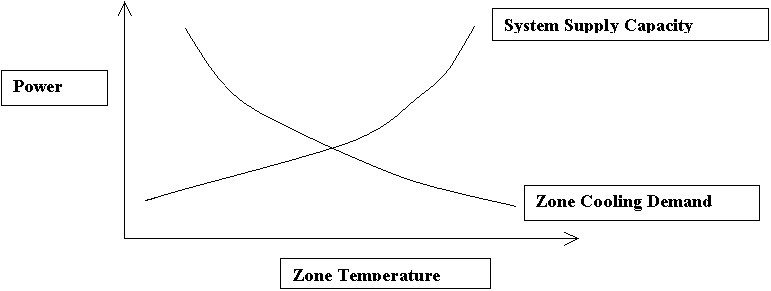
\includegraphics[width=0.9\textwidth, height=0.9\textheight, keepaspectratio=true]{media/image7.png}
\caption{Sequential Simulation Supply/Demand Relationship. \protect \label{fig:sequential-simulation-supplydemand}}
\end{figure}

However, in most situations the system capacity is dependent on outside conditions and/or other parameters of the conditioned space. The simple supply and demand situation above becomes a more complex relationship and the system curve is not fixed. The solution should move up and down the demand curve. This doesn't happen in sequential simulation methods and the lack of feedback from the system to the building can lead to nonphysical results. For example, if the system provides too much cooling to a conditioned space the excess is reported by the program as ``overcooling''. Other categories of unmatched loads exist and are similarly reported by the program. While this kind of reporting enables the affected system or plant components to be properly sized, the system designer would, in most cases, prefer to see the actual change in zone temperature. The same mismatches can occur between the system and plant simulations when they are simulated sequentially.

To obtain a simulation that is physically realistic, the elements have to be linked in a simultaneous solution scheme. The entire integrated program can be represented as a series of functional elements connected by fluid loops as shown in Figure ``Schematic of Simultaneous Solution Scheme''. In EnergyPlus all the elements are integrated and controlled by the Integrated Solution Manager. The loops are divided into supply and demand sides, and the solution scheme generally relies on successive substitution iteration to reconcile supply and demand using the Gauss-Seidell philosophy of continuous updating.

\begin{figure}[hbtp] % fig 4
\centering
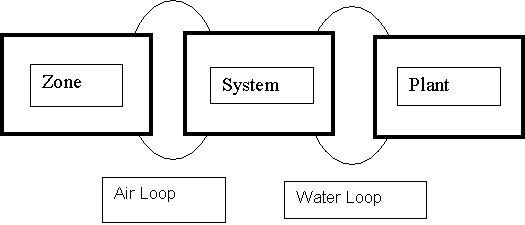
\includegraphics[width=0.9\textwidth, height=0.9\textheight, keepaspectratio=true]{media/image8.png}
\caption{Schematic of Simultaneous Solution Scheme \protect \label{fig:schematic-of-simultaneous-solution-scheme}}
\end{figure}

In the sections which follow, the various individual functions of the integrated solution will be described.
